\section{Task 2}
Hello whowhwonsifjdifnsdjif ni %adding example text with lorem ipsum

\begin{figure}[h] %example of figure with picture 'h' tells latex to place it 'around' here
	\centering
	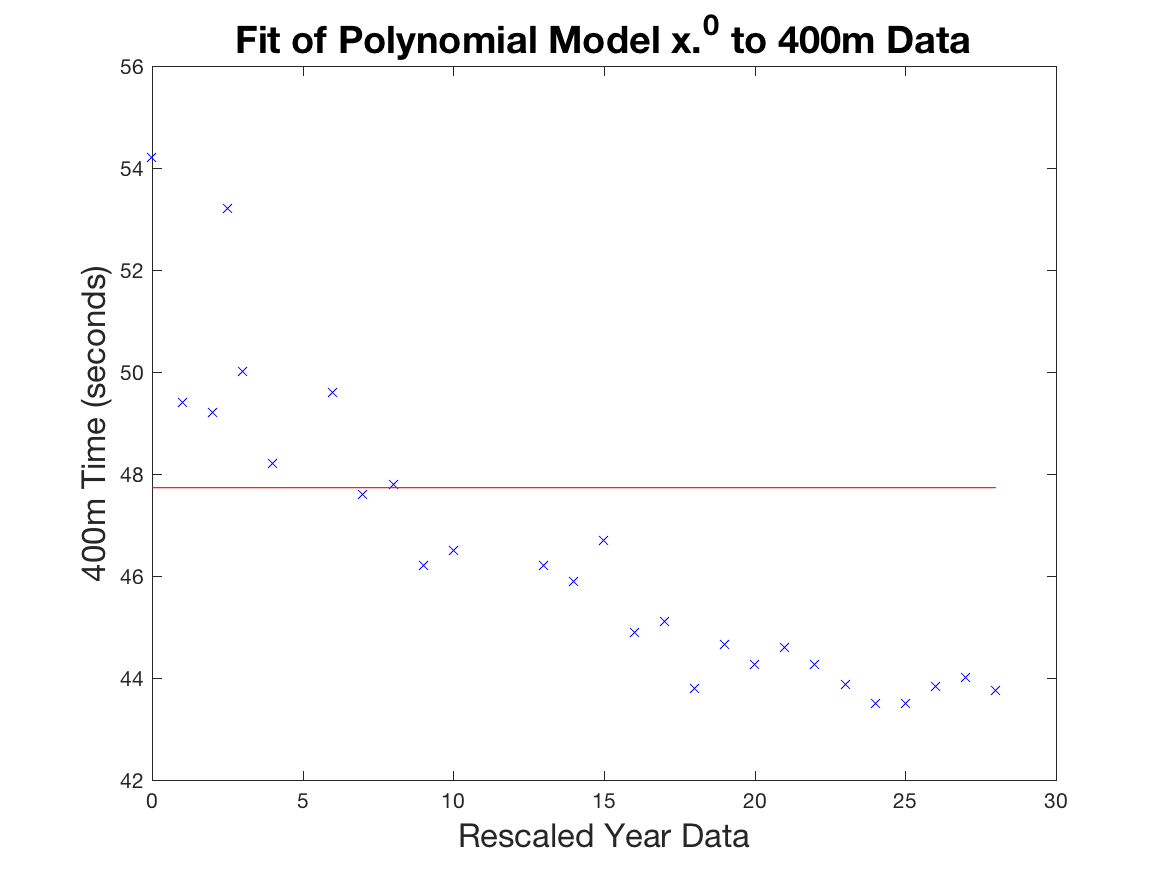
\includegraphics[width=0.7\textwidth]{model0.png} % replace TeamWin.png with image filename and save file in ../images
	\caption{Team win in action!}
	\label{teamWin} % use descriptive labels so can reference in text
\end{figure}

Figure \ref{teamWin} Shows how much fun we will have.

In task 2 we are given the task to find the value of $\lambda$ that gives the 'best' predictive performance on the Olympic men's 100m data using 5-fold cross-validation.

\begin{figure}[h] %example of figure with picture 'h' tells latex to place it 'around' here
	\centering
	\begin{subfigure}{.5\textwidth}
		content...
	\end{subfigure}
	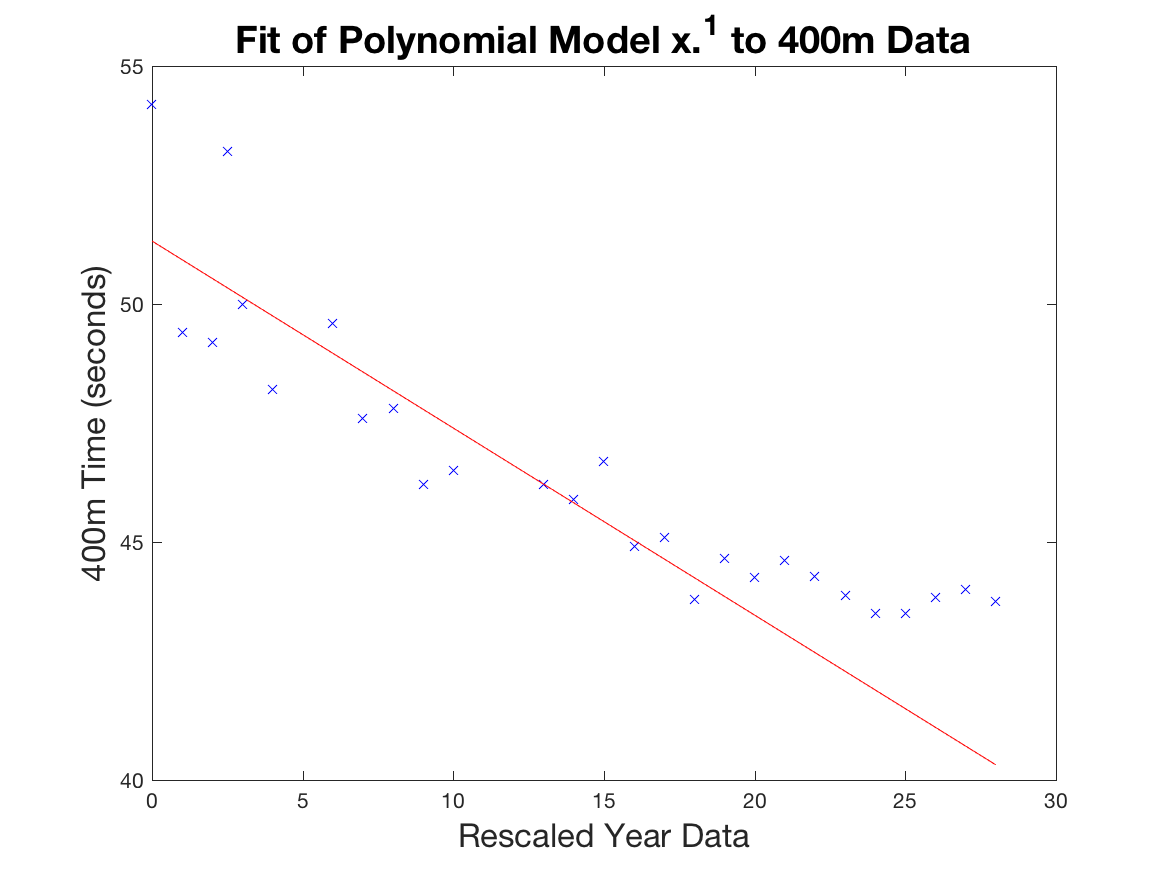
\includegraphics[width=0.7\textwidth]{model1.png} % replace TeamWin.png with image filename and save file in ../images
	\caption{Team win in action!}
	\label{teamWin} % use descriptive labels so can reference in text
\end{figure}

\lipsum[1-4]


